\documentclass[a4paper,11pt]{article}
\usepackage{amsmath,amsthm,amsfonts,amssymb,amscd,amstext,vmargin,graphics,graphicx,tabularx,multicol} \usepackage[french]{babel}
\usepackage[utf8]{inputenc}  
\usepackage[T1]{fontenc} 
\usepackage[T1]{fontenc}
\usepackage{amsmath,amssymb}
\usepackage{pstricks-add,tikz,tkz-tab,variations}
\usepackage[autolanguage,np]{numprint} 

\setmarginsrb{1.5cm}{0.5cm}{1cm}{0.5cm}{0cm}{0cm}{0cm}{0cm} %Gauche, haut, droite, haut
\newcounter{numexo}
\newcommand{\exo}[1]{\stepcounter{numexo}\noindent{\bf Exercice~\thenumexo} : \marginpar{\hfill /#1}}
\reversemarginpar


\newcounter{enumtabi}
\newcounter{enumtaba}
\newcommand{\q}{\stepcounter{enumtabi} \theenumtabi.  }
\newcommand{\qa}{\stepcounter{enumtaba} (\alph{enumtaba}) }
\newcommand{\initq}{\setcounter{enumtabi}{0}}
\newcommand{\initqa}{\setcounter{enumtaba}{0}}

\newcommand{\be}{\begin{enumerate}}
\newcommand{\ee}{\end{enumerate}}
\newcommand{\bi}{\begin{itemize}}
\newcommand{\ei}{\end{itemize}}
\newcommand{\bp}{\begin{pspicture*}}
\newcommand{\ep}{\end{pspicture*}}
\newcommand{\bt}{\begin{tabular}}
\newcommand{\et}{\end{tabular}}
\renewcommand{\tabularxcolumn}[1]{>{\centering}m{#1}} %(colonne m{} centrée, au lieu de p par défault) 
\newcommand{\tnl}{\tabularnewline}

\newcommand{\trait}{\noindent \rule{\linewidth}{0.2mm}}
\newcommand{\hs}[1]{\hspace{#1}}
\newcommand{\vs}[1]{\vspace{#1}}

\newcommand{\N}{\mathbb{N}}
\newcommand{\Z}{\mathbb{Z}}
\newcommand{\R}{\mathbb{R}}
\newcommand{\C}{\mathbb{C}}
\newcommand{\Dcal}{\mathcal{D}}
\newcommand{\Ccal}{\mathcal{C}}
\newcommand{\mc}{\mathcal}

\newcommand{\vect}[1]{\overrightarrow{#1}}
\newcommand{\ds}{\displaystyle}
\newcommand{\eq}{\quad \Leftrightarrow \quad}
\newcommand{\vecti}{\vec{\imath}}
\newcommand{\vectj}{\vec{\jmath}}
\newcommand{\Oij}{(O;\vec{\imath}, \vec{\jmath})}
\newcommand{\OIJ}{(O;I,J)}

\newcommand{\bmul}[1]{\begin{multicols}{#1}}
\newcommand{\emul}{\end{multicols}}


\newcommand{\reponse}[1][1]{%
\multido{}{#1}{\makebox[\linewidth]{\rule[0pt]{0pt}{20pt}\dotfill}
}}

\newcommand{\titre}[5] 
% #1: titre #2: haut gauche #3: bas gauche #4: haut droite #5: bas droite
{
\noindent #2 \hfill #4 \\
#3 \hfill #5

\vspace{-1.6cm}

\begin{center}\rule{6cm}{0.5mm}\end{center}
\vspace{0.2cm}
\begin{center}{\large{\textbf{#1}}}\end{center}
\begin{center}\rule{6cm}{0.5mm}\end{center}
}



\begin{document}
\pagestyle{empty}
\titre{Contrôle 2 : Fractions (Chp 1 et 2), probabilités et symétrie centrale }{Nom :}{Prénom :}{Classe}{Date}



\exo{5}

Calculer les expressions suivantes en détaillant toutes vos étapes de calculs et \textbf{simplifier} les résultats si besoin :

\bmul{4}

$R = \dfrac{4}{5} + \dfrac{18}{5}$\\


\columnbreak

$E = \dfrac{5}{3} - \dfrac{10}{12}$\\ 


\columnbreak

$P = 3 - \dfrac{2}{7}$\\ 

\columnbreak

$S =\dfrac{1}{3}+\dfrac{4}{5} - \dfrac{11}{45}$\\ 

\emul

\vspace*{0.5cm}

\exo{2}

Dans une carafe d'un litre, on mélange $\dfrac{1}{2}$ L de jus d'orange, $\dfrac{1}{20}$ L de jus de citron, $\dfrac{1}{10}$ L de jus de pamplemousse et $\dfrac{2}{5}$ L de sucre de canne.\\

Quelle quantité de boisson obtient-on ? La carafe va-t-elle déborder ? Pourquoi ?(\textbf{Justifier votre réponse par des calculs.)}\\

\vspace*{0.5cm}

\exo{2,5}

On prend deux dés cubiques non truqués. On les lance et on ajoute les deux nombres obtenus.\\

\initq \q Est-ce une expérience aléatoire ? (\textbf{Justifier votre réponse)}\\

\q Combien y a-t-il d'issues possibles ? Citer-les.\\

\vspace*{0.5cm}

\exo{1}

Lucie dit qu'elle a lancé six fois de suite un dé à six faces non truqué et elle affirme qu'elle a obtenu à chaque fois le chiffre 5.\\

\initq \q Est-ce possible ?(\textbf{Justifier votre réponse)}\\

\q Si Lucie relance le dé, a-t-elle une chance de refaire un 5.(\textbf{Justifier votre réponse)}\\

\vspace*{0.5cm}

\exo{1,5} 

\bmul{2}
Pour gagner à ce jeu, il faut tomber sur la couleur rouge. On a le choix entre une roulette, un dé et une urne contenant dix boules.\\

Que faut-il choisir pour avoir le plus de chance de gagner : la roulette, le dé ou l'urne ? (\textbf{Justifier votre réponse en prenant appui sur votre cours de probabilité.})\\
\columnbreak


\includegraphics[scale=1]{jeuouge.eps} 

\emul



\vspace*{0.5cm}



\newpage

\exo{2} Dans la figure ci-dessous, les quadrilatères ACBD et EFHG sont symétriques par rapport au point O.

\begin{center}
 \includegraphics[scale=1]{quadrilatere.eps}\\
 \end{center} 

\initq
\q Quel est le symétrique de point B par rapport au point O.\\

\q Quel est le symétrique du segment [AD] par rapport au point O.\\

\q Quel est le symétrique de la droite (FH) par rapport au point O.\\

\q Quel est le symétrique de la droite (FG) par rapport au point O.\\

\vspace*{0.5cm}

\exo{2}

Après avoir reproduit ce dessin sur \textbf{ta copie}, complète-le en faisant le symétrique de chaque figure par rapport au point O.\\

\begin{center}
\includegraphics[scale=1]{figure.eps} 
\end{center}

\vspace*{0.5cm}

\exo{4}

\initq 
\q Construire un triangle ABC rectangle en A tel que  : AB = 5cm et AC = 3cm.\\

\q Construire sur la même figure en utilisant trois couleurs différentes, les triangles symétriques du triangle ABC par rapport : 

\bmul{3}
a. au point A

\columnbreak

b. au point B
\columnbreak

c. au point C
\emul


\end{document}
